\documentclass[12pt]{article}
\usepackage[left=2cm,right=2cm,top=2cm,bottom=2cm,bindingoffset=0cm]{geometry}
\usepackage{hyperref}
\usepackage{fontspec}
\usepackage{polyglossia}
\setdefaultlanguage{russian}
\pagestyle{empty}
\setmainfont[Mapping=tex-text]{CMU Serif}

\begin{document}
%% Весь этот текст можно удалить
%% ====== от сих =====
\centering {\LARGE Формальные языки}

{\Large Контрольная работа 1, вариант 1}
\bigskip

\begin{enumerate}
  \item Построить минимальный детерминированный конечный автомат для языка \\ $L = \{ \omega \in \{ 0, 1, \dots, 9 \}^* \, | \, \omega = 0 (mod \, 25) \} $
  \item { 
         Построить автомат, распознающий объединение языков, распознаваемых следующими автоматами
         
         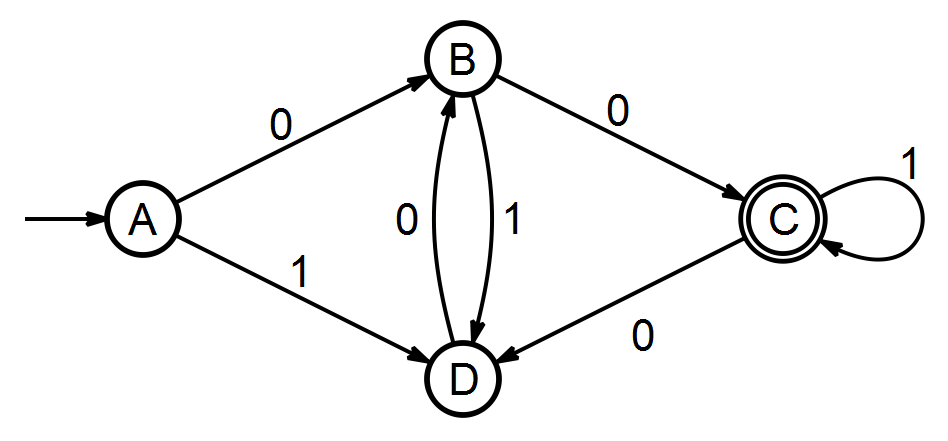
\includegraphics[width=250pt]{../../2016_spr/05.03/2_0.png}
         
~\\~
         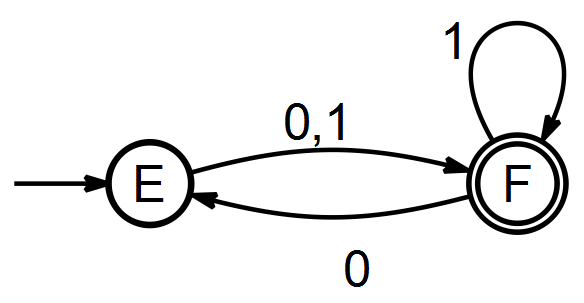
\includegraphics[width=150pt]{../../2016_spr/05.03/2_1.png} 
        }
    \item Построить регулярную грамматику, задающую язык \\ $L = \{ a \omega b \, | \, \omega \in \{ 0, 1 \}^*; a, b \in \{ 0, 1 \}; a \, xor \, b = 1 \} $
    \item Проверить регулярность языка арифметических выражений (операции +, *) в префиксной записи. Если язык регулярный --- привести грамматику, автомат или регулярное выражение, его задающее. Если нет --- привести доказательство
    \item {Построить эпсилон-замыкание автомата
           
           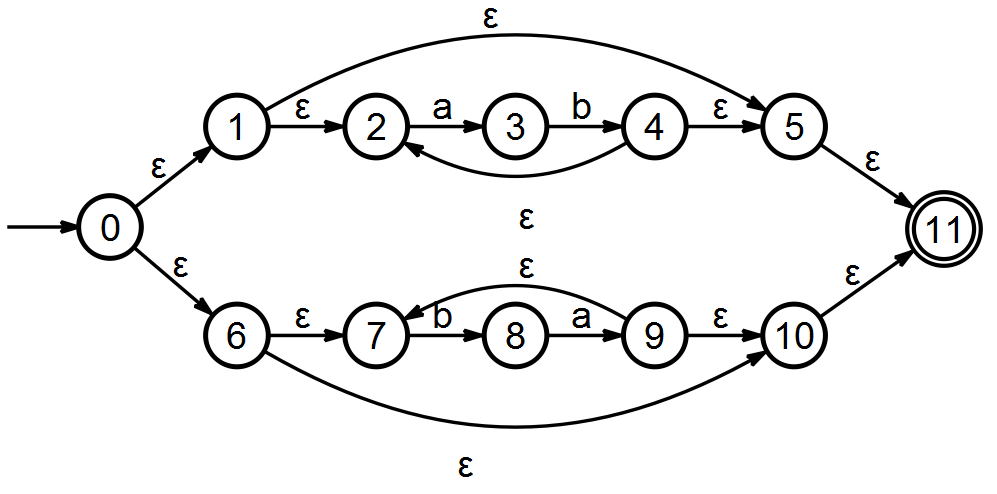
\includegraphics[width=0.7\textwidth]{test1a_ec.PNG}
    }
\end{enumerate}

\pagebreak

\centering {\LARGE Формальные языки}

{\Large Контрольная работа 1, вариант 2}
\bigskip

\begin{enumerate}
  \item Построить минимальный детерминированный конечный автомат для языка \\ $L = \{ \omega a b \, | \, \omega \in \{ 0, 1, \dots, 9 \}^*; a, b \in \{ 0, 1, \dots, 9 \}; a + b = 5 \} $
  \item { 
         Построить автомат, распознающий разность языков, распознаваемых следующими автоматами
         
         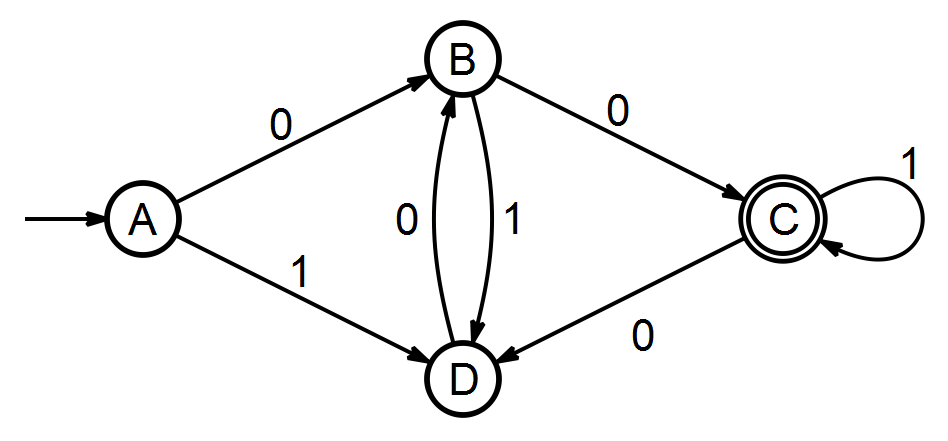
\includegraphics[width=250pt]{../../2016_spr/05.03/2_0.png}
         
~\\~
         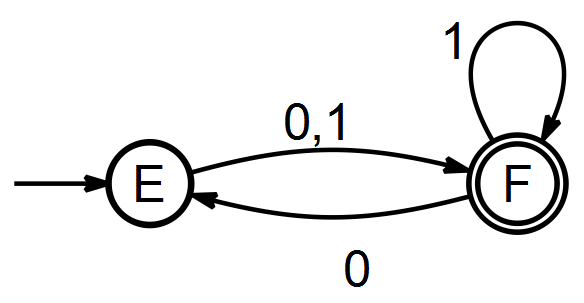
\includegraphics[width=150pt]{../../2016_spr/05.03/2_1.png} 
        }
    \item Построить регулярную грамматику, задающую язык \\ $L = \{ a \omega b \, | \, \omega \in \{ 0, 1 \}^*; a, b \in \{ 0, 1 \}; a \, xor \, b = 0 \} $
    \item Проверить регулярность языка арифметических выражений (операции +, *) в постфиксной записи. Если язык регулярный --- привести грамматику, автомат или регулярное выражение, его задающее. Если нет --- привести доказательство
    \item {Построить эпсилон-замыкание автомата
           
           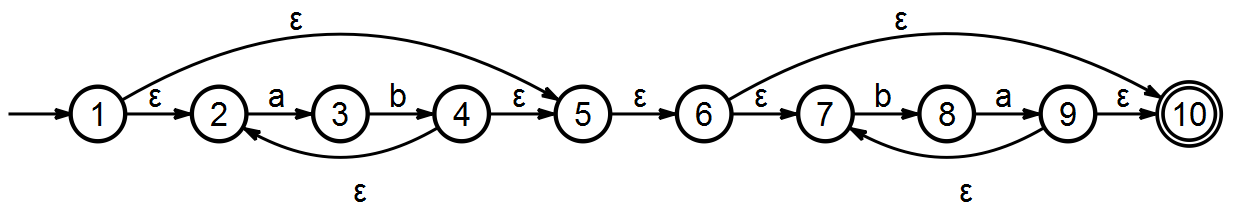
\includegraphics[width=0.9\textwidth]{test1b_ec.PNG}
    }
\end{enumerate}

\pagebreak 

\begin{document}
%% Весь этот текст можно удалить
%% ====== от сих =====
\centering {\LARGE Формальные языки}

{\Large Контрольная работа 1, попытка 2, вариант 1}
\bigskip

\begin{enumerate}
  \item Построить минимальный детерминированный конечный автомат для языка \\ $L = \{ \alpha \omega \beta \, | \, \alpha, \beta \in \{ 0, 1, \dots, 9 \}^*; \omega \in \{ 0, 1 \}; |\omega| = 3, \omega$ --- двоичная запись простого числа$\}$
  \item { 
         Построить автомат, распознающий числа, кратные 6}
    \item Построить регулярную грамматику, задающую язык \\ $L = \{ \alpha a \beta b \gamma \, | \, \alpha, \beta, \gamma \in \{ 0, 1 \}^*; |\beta| = 3; a, b \in \{ 0, 1 \}; a \, and \, b = 0 \} $
    \item Проверить регулярность языка $\{ \omega \bar \omega \, | \, \omega \in \{0, 1\}^* \}$, где $\bar \omega$ получена заменой символов $0$ на $1$ и наоборот ($\overline{001} = 110$). Если язык регулярный --- привести грамматику, автомат или регулярное выражение, его задающее. Если нет --- привести доказательство
    \item {Построить недетерминированный автомат по регулярному выражению $ (ab)^*a^*ba  $, построить эпсилон-замыкание автомата}
    
\end{enumerate}

\bigskip

~\\~

\bigskip

\rule{\textwidth}{1pt}

\bigskip

~\\~\\~

\bigskip

\centering {\LARGE Формальные языки}

{\Large Контрольная работа 1, попытка 2, вариант 2}
\bigskip

\begin{enumerate}
  \item Построить минимальный детерминированный конечный автомат для языка \\ $L = \{ \alpha \omega \beta \, | \, \alpha, \beta \in \{ 0, 1, \dots, 9 \}^*; \omega \in \{ 0, 1 \}; |\omega| = 3, \omega$ --- двоичная запись целого числа, не являющегося простым$\}$
  \item { 
         Построить автомат, распознающий числа, кратные 15}
    \item Построить регулярную грамматику, задающую язык \\ $L = \{ \alpha a \beta b \gamma \, | \, \alpha, \beta, \gamma \in \{ 0, 1 \}^*; |\beta| = 3; a, b \in \{ 0, 1 \}; a \, or \, b = 1 \} $
    \item Проверить регулярность языка $\{ \omega \omega \, | \, \omega \in \{0, 1\}^* \}$. Если язык регулярный --- привести грамматику, автомат или регулярное выражение, его задающее. Если нет --- привести доказательство
    \item {Построить недетерминированный автомат по регулярному выражению $ (ab)b^*(ba)^*  $, построить эпсилон-замыкание автомата }
\end{enumerate}
\end{document}
